\documentclass[tikz,border=2mm]{standalone}
\begin{document}
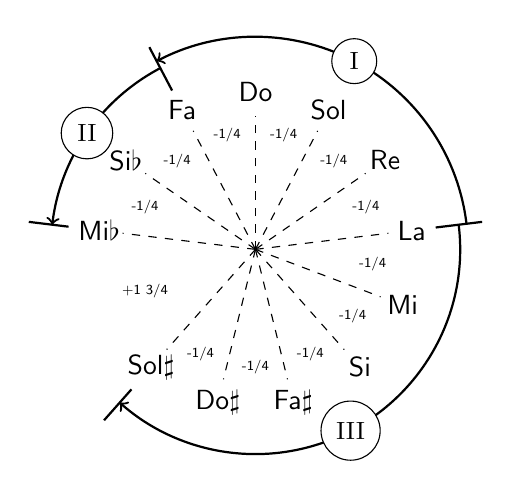
\begin{tikzpicture}
\newcommand{\myangle}{27.6923}
\foreach \nota/\text [count=\sector] in {Mib/Mi$\flat$,Sib/Si$\flat$,Fa/Fa,Do/Do,Sol/Sol,Re/Re,La/La, Mi/Mi,Si/Si,Fas/Fa$\sharp$,Dos/Do$\sharp$,Sols/Sol$\sharp$} 
    {
        \draw[dashed, shorten >=3mm] (0,0) -- ++({(4-\sector)*\myangle+90}:2cm) node[font=\sffamily] (\nota) {\text};
    }

\foreach \i [count=\xi] in {1,2,...,11}
    {
        \path (0,0) -- ++({(3.5-\xi)*\myangle+90}:15mm) node[font=\tiny\sffamily]  {-1/4};
    }
\path (0,0) -- ++({4*\myangle+90}:15mm) node[font=\tiny\sffamily]  {+1 3/4};


\draw[thick] (Mib)--++({90+3*\myangle}:9mm);
\draw[thick] (Fa)--++({90+\myangle}:9mm);
\draw[thick] (La)--++({90-3*\myangle}:9mm);
\draw[thick] (Sols)--++({90-8*\myangle}:9mm);

\draw[->,thick] ({90+\myangle}:26mm) arc [start angle={90+\myangle}, delta angle={2*\myangle}, radius=26mm]; 
\node[draw, circle, fill=white, font=\small] at (90+2*\myangle:26mm) {II};

\draw[->,thick] ({90-3*\myangle}:27mm) arc [start angle={90-3*\myangle}, delta angle={4*\myangle}, radius=27mm]; 
\node[draw, circle, fill=white, font=\small] at (90-\myangle:27mm) {I};

\draw[->,thick] ({90-3*\myangle}:26mm) arc [start angle={90-3*\myangle}, delta angle={-5*\myangle}, radius=26mm]; 
\node[draw, circle, fill=white, font=\small] at (90-5.5*\myangle:26mm) {III};
\end{tikzpicture}
\end{document}